\documentclass[tikz]{standalone}

\usetikzlibrary{arrows.meta,positioning}

\begin{document}
	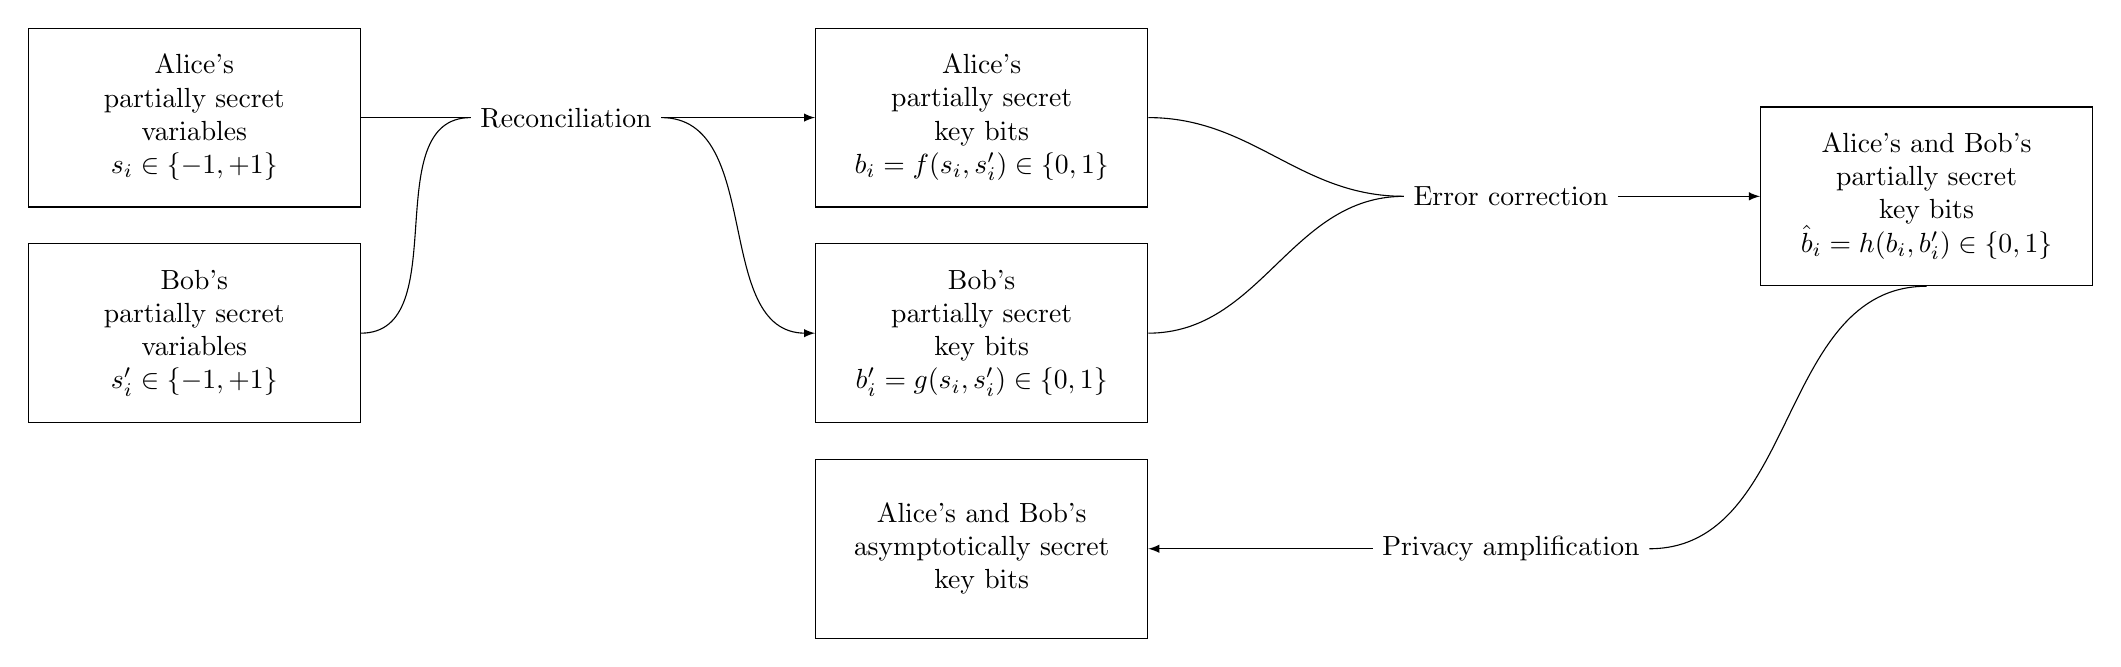
\begin{tikzpicture}[
		node distance=3ex,
		arrow/.style={-latex},
		block/.style={draw, minimum height=15ex, minimum width=12em, align=center},
	]
		\node (av) [block] {Alice's\\partially secret\\variables\\$s_i\in\{-1,+1\}$};
		\node (bv) [block, below=of av] {Bob's\\partially secret \\variables\\$s^\prime_i\in\{-1,+1\}$};
		\node (ab) at (10,-1|-av) [block] {Alice's\\partially secret\\key bits\\$b_i=f(s_i,s_i^\prime)\in\{0,1\}$};
		\node (bb) [block, below=of ab] {Bob's\\partially secret\\key bits\\$b_i^\prime=g(s_i,s_i^\prime)\in\{0,1\}$};
		\node (ps) at (22,-1) [block] {Alice's and Bob's\\partially secret\\key bits\\$\hat{b}_i=h(b_i,b_i^\prime)\in\{0,1\}$};

		\node (rec) at ([xshift=-9em]ab.west) {Reconciliation};
		
		\draw (av.east) to[out=0, in=180] (rec);
		\draw (bv.east) to[out=0, in=180] (rec);
		\draw[arrow] (rec) -- (ab.west);
		\draw[arrow] (rec) to[out=0, in=180] (bb.west);
		
		\node (eec) at ([xshift=-9em]ps.west) {Error correction};
		\draw (ab.east) to[out=0, in=180] (eec);
		\draw (bb.east) to[out=0, in=180] (eec);
		\draw[arrow] (eec) -- (ps.west);
		
		\node (as) [block, below=of bb] {Alice's and Bob's\\asymptotically secret\\key bits};
		\node (pa) at (as-|eec) {Privacy amplification};
		\draw (ps.south) to[out=180, in=0] (pa.east);
		\draw[arrow] (pa.west) -- (as);
	\end{tikzpicture}
\end{document}
